\documentclass[a4paper]{article}
\usepackage[a4paper, top=8mm, bottom=8mm, left=8mm, right=8mm]{geometry}
\usepackage{polyglossia}
\setdefaultlanguage[babelshorthands=true]{russian}
\setotherlanguage{english}
\usepackage{fontspec}
\setmainfont{FreeSerif}
\newfontfamily{\russianfonttt}[Scale=0.7]{DejaVuSansMono}
\usepackage[tiny, compact]{titlesec}
\usepackage{titling}
\setlength{\droptitle}{-1cm}
\pretitle{\begin{center}\begin{bfseries}\Large}
\posttitle{\par\end{bfseries}\end{center}}
\preauthor{\begin{center}\normalsize}
\postauthor{\par\end{center}\vspace{-1.8cm}}
\usepackage{hyperref}
\usepackage{bookmark}
\usepackage{csquotes}
\usepackage{enumitem}
\usepackage{graphicx}
\usepackage{amsmath}

\title{Реализация свёртки изображений на Python}
\author{Сапегин Павел Николаевич}
\date{}

\begin{document}
\maketitle
\begin{flushright}
\begin{tabular}{r}
    Группа: \emph{\enquote{25.Б41-мм}} \\
    Кафедра: \emph{кафедра системного программирования} \\
    Научный руководитель: \emph{Пономарев Николай Алексеевич} \\
    Номер семестра практики: \emph{2} \\
\end{tabular}
\end{flushright}

\section{Введение}

Свёртка~--- одна из ключевых операций в обработке изображений и компьютерном зрении. Она применяется для размытия, повышения резкости, выделения границ и других преобразований. Математически свёртка изображения $I$ с ядром $K$ размера $(2p+1) \times (2p+1)$ определяется как:
\[
(I * K)[i, j] = \sum_{m=-p}^{p} \sum_{n=-p}^{p} I[i+m,\, j+n] \cdot K[m, n]
\]

В рамках учебной практики предлагается реализовать данную операцию на языке Python, а затем сравнить производительность реализации с библиотеками OpenCV и Pillow.

\section{Постановка задачи}

\textbf{Целью работы является} реализация операции свёртки изображений на языке Python, а также её тестирование и сравнение производительности с решениями на основе библиотек OpenCV и Pillow.

\textbf{Задачи:}
\begin{itemize}
    \item Реализовать функцию свёртки для полутоновых и цветных (RGB) изображений с опциональным переводом в оттенки серого.
    \item Реализовать несколько режимов дополнения (обработка краёв): \verb|valid|, \verb|zero|, \verb|edge|, \verb|reflect|.
    \item Подготовить набор стандартных ядер: \verb|identity|, \verb|blur|, \verb|gaussian_blur|, \verb|sharpen|, \verb|edge|.
    \item Покрыть реализацию тестами с использованием эталонных изображений.
    \item Провести тест производительности и сравнить скорость выполнения с OpenCV и Pillow.
\end{itemize}

\section{Описание предлагаемого решения}

\subsection{Перевод в оттенки серого}

Функция \verb|to_grayscale| переводит RGB-изображение в одноканальное (оттенки серого) по стандартной взвешенной формуле яркости:
\[
Y = 0{,}299 \cdot R + 0{,}587 \cdot G + 0{,}114 \cdot B
\]

Коэффициенты соответствуют стандарту BT.601 и учитывают восприятие цветов человеческим глазом. Вычисления выполняются поэлементно на массиве NumPy без циклов.

\subsection{Режимы дополнения (padding)}

Поскольку применение ядра к граничным пикселям требует данных за пределами изображения, реализованы четыре режима дополнения:

\begin{itemize}
    \item \textbf{valid}~--- дополнение не производится; результат меньше исходного изображения на \(2p\) пикселей по каждой стороне, где \(p\)~--- это размер отбрасываемой рамки (в пикселях).
    \item \textbf{zero}~--- граничные пиксели дополняются нулями (чёрный цвет).
    \item \textbf{edge}~--- граничные пиксели копируются от ближайшего края изображения (\verb|BORDER_REPLICATE| в терминологии OpenCV).
    \item \textbf{reflect}~--- производится зеркальное отражение пикселей относительно края (при этом крайний пиксель не дублируется, аналог \verb|BORDER_REFLECT| в OpenCV).
\end{itemize}

Режимы \verb|edge| и \verb|reflect| реализованы функциями \verb|apply_edge_padding| 
и \verb|apply_reflect_padding|, которые заполняют граничные полосы нового массива NumPy 
увеличенного размера.
\subsection{Функция свёртки}

Основная функция, \verb|conv|, принимает PIL-изображение, ядро, режим дополнения и флаг перевода в серый. Алгоритм работает следующим образом:

\begin{enumerate}
    \item При необходимости изображение переводится в оттенки серого.
    \item Изображение преобразуется в массив NumPy.
    \item В зависимости от режима обработки краёв формируется дополненный массив \verb|padded_img| и нулевой массив результата \verb|result| нужного размера.
    \item Свёртка выполняется циклом по элементам ядра: на каждой итерации выделяется срез дополненного изображения нужного размера и поэлементно прибавляется к результату, умноженный на соответствующий элемент ядра.
    \item Значения результата ограничиваются диапазоном $[0, 255]$ и приводятся к типу \verb|uint8|.
\end{enumerate}

\subsection{Ядра фильтров}

В словаре \verb|FILTERS| определены следующие ядра $3 \times 3$:

\begin{itemize}
    \item \textbf{identity}~--- единичное ядро, оставляет изображение без изменений.
    \item \textbf{blur}~--- равномерное усредняющее ядро (box blur), каждый элемент равен $\tfrac{1}{9}$.
    \item \textbf{gaussian\_blur}~--- аппроксимация гауссова размытия с весами $1{:}2{:}1$.
    \item \textbf{sharpen}~--- ядро повышения резкости с центральным весом $5$ и отрицательными соседями $-1$.
    \item \textbf{edge}~--- ядро выделения границ с центральным весом $8$ и соседями $-1$.
\end{itemize}

\subsection{Интерфейс командной строки}

Модуль \verb|main.py| содержит точку входа с аргументами \verb|input|, \verb|output|, \verb|--filter|, \verb|--padding| и \verb|--gray|, что позволяет применять фильтры к произвольным изображениям без написания кода.

\section{Тестирование}

\subsection{Функциональные тесты}

Тесты в файле \verb|test_conv.py| используют метод эталонных изображений: для каждой комбинации ядра, режима дополнения и цветового режима эталонное изображение было заранее получено 
с помощью библиотеки OpenCV. При запуске теста результат функции \verb|conv| поэлементно сравнивается с эталоном с помощью \verb|np.testing.assert_array_equal|, что гарантирует побитовое совпадение. Тестируются 8 комбинаций параметров для RGB-изображений и изображений в оттенках серого, а также отдельно функция \verb|to_grayscale|.
Эксперименты проводились на системе со следующими характеристиками: 
\textit{процессор} Intel Core i5-13420H, \textit{ОЗУ} 16~ГБ,\ \textit{ОС} Ubuntu 24.04.4.
\subsection{Тест производительности}

Тест производительности в файле \verb|test_benchmark.py| использует библиотеку \verb|pytest-benchmark| и сравнивает три реализации:
\begin{itemize}
    \item \textbf{custom}~--- реализация из \verb|main.py|.
    \item \textbf{opencv}~--- функция \verb|cv2.filter2D| с аналогичными параметрами.
    \item \textbf{pillow}~--- класс \verb|ImageFilter.Kernel| из библиотеки Pillow.
\end{itemize}
Тесты запускаются на случайных изображениях размерами $128\times128$, $512\times512$, $1024\times1024$ и $4096\times4096$ пикселей для всех сочетаний ядра (\verb|sharpen|, \verb|blur|, \verb|edge|), режима padding (\verb|zero|, \verb|edge|, \verb|reflect|) и цветового режима (RGB / оттенки серого).

Результаты теста производительности визуализируются скриптом \verb|visualisation.py| и представлены на рисунке~\ref{fig:bench}.

\begin{figure}[h]
    \centering
    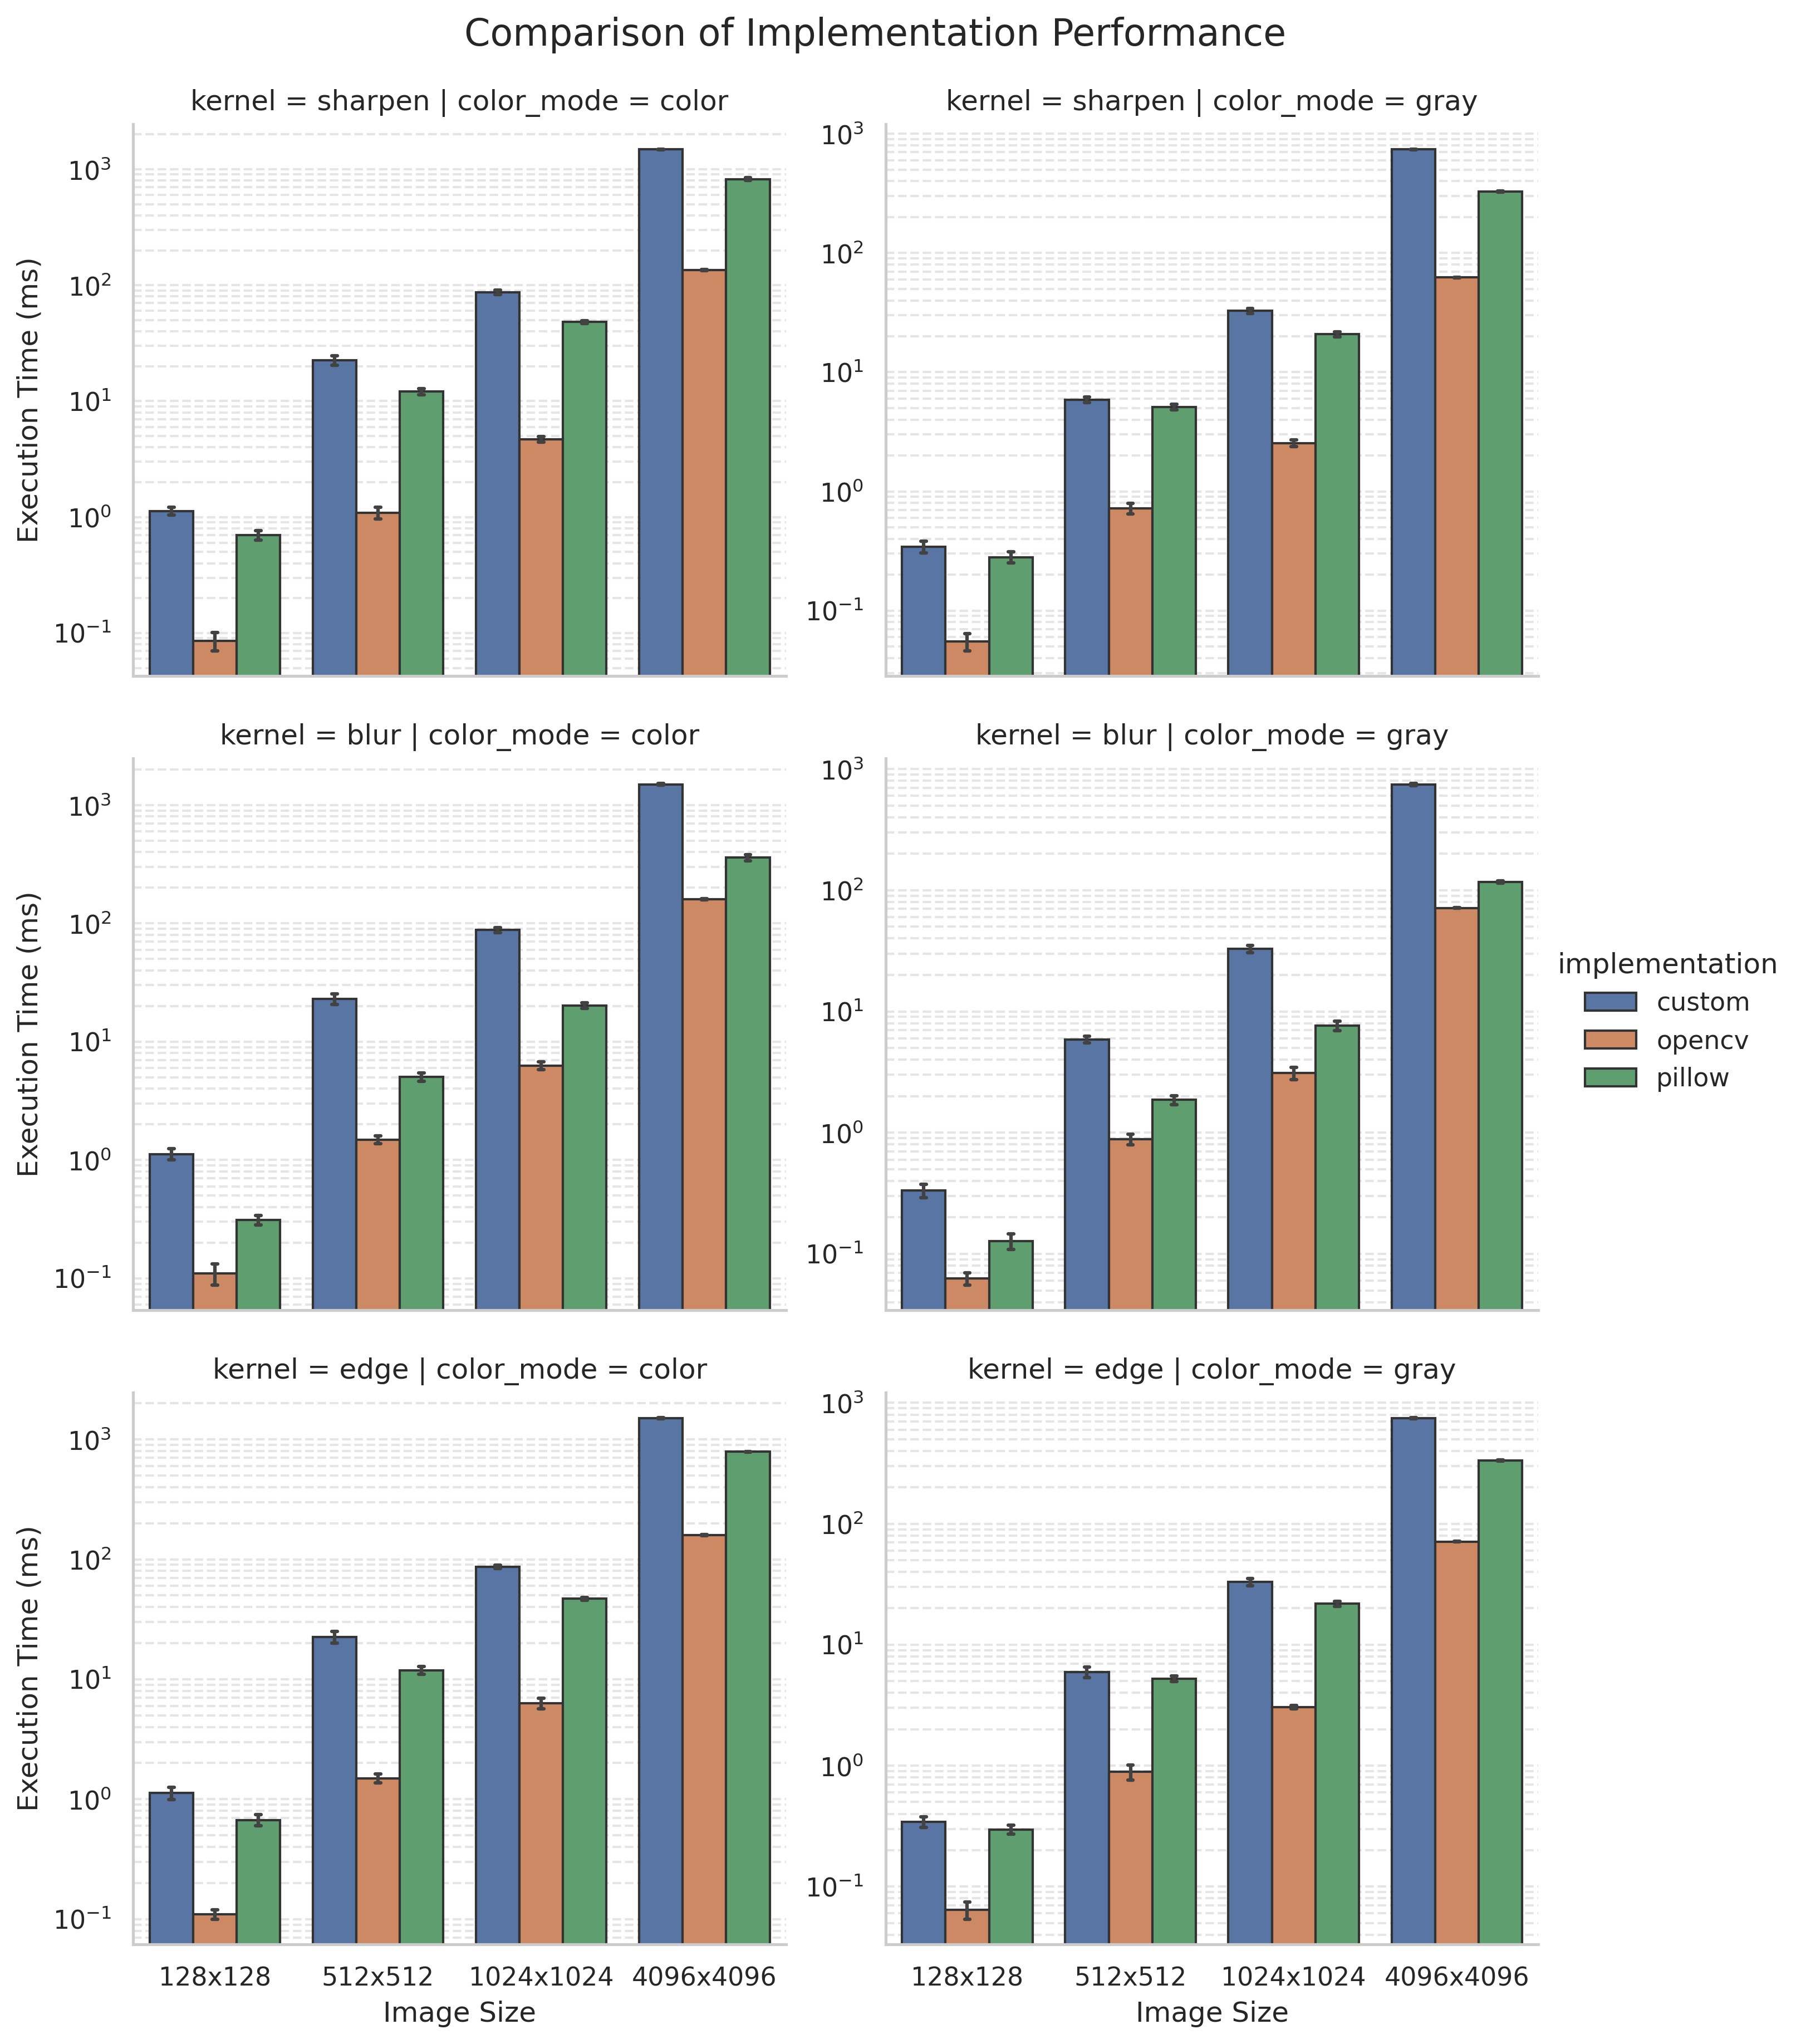
\includegraphics[width=\textwidth]{bench_results.png}
    \caption{Сравнение времени выполнения свёртки для трёх реализаций. Ось Y~--- логарифмическая. Планки погрешностей соответствуют стандартному отклонению по запускам.}
    \label{fig:bench}
\end{figure}

Как видно из графиков, реализация на OpenCV является наиболее быстрой во всех конфигурациях: на изображении $4096\times4096$ она выполняет свёртку примерно на 1--2 порядка быстрее пользовательской реализации. Реализация на Pillow занимает промежуточное положение. Пользовательская реализация (custom) заметно медленнее оптимизированных библиотек, поскольку всё же выполняет цикл на уровне Python по элементам ядра. При переходе к изображениям в оттенках серого время выполнения для всех реализаций уменьшается примерно в 3 раза (по числу каналов), что соответствует ожиданиям.

В ходе выполнения работы получены следующие результаты:
\begin{itemize}
    \item Реализована операция свёртки изображений на Python с поддержкой четырёх режимов дополнения и обработки RGB-изображений и изображений в оттенках серого.
    \item Реализован набор стандартных ядер: \verb|identity|, \verb|blur|, \verb|gaussian_blur|, \verb|sharpen|, \verb|edge|.
    \item Написаны функциональные тесты на основе эталонных изображений, подтверждающие корректность реализации.
    \item Проведён тест производительности, показавший, что пользовательская реализация корректна, однако уступает по скорости оптимизированным библиотекам OpenCV и Pillow, что объясняется отсутствием низкоуровневых оптимизаций.
\end{itemize}

Репозиторий с реализацией: \url{https://github.com/PavelSapegin/image_conv}.
\end{document}
